%%%%%%%%%%%%%%%%%%%%%%%%%%%%%%%%%%%%%%%%%%%%%%%%%%%%%%%%%%%%%%%%%%%%%%%%%%%%%%%%
% NFO-VOS poster, A0 portrait (TUM template, Vorlagen/PlakatA0Hoch.tex).
% Compile from this directory:  latexmk -pdf NFO_VOS_poster
% Content: NFO_VOS_inhalt.tex. Figures: plots/nfo/ (benchmark/nfo_vos/tools/poster_figures.py).
% Board is 80 cm wide: print A0 at 100 % and trim ~2 cm per side (content starts ~4.6 cm from each edge).
% Not in git (third-party, see .gitignore): the TUM template (Ressourcen/ incl. the logo row edited in
% Ressourcen/Plakat/Anfang.tex, _Einstellungen.tex) and plots/logos/ (AIT trimmed, MCML as PDF, TUM).
%%%%%%%%%%%%%%%%%%%%%%%%%%%%%%%%%%%%%%%%%%%%%%%%%%%%%%%%%%%%%%%%%%%%%%%%%%%%%%%%

\PassOptionsToPackage{english,ngerman}{babel} % English hyphenation, selected after \begin{document}
\input{./Ressourcen/Plakat/PraeambelA0Hoch.tex} % !!! NICHT ENTFERNEN !!!
\input{./_Einstellungen.tex}                    % !!! DATEI ANPASSEN !!!

\usepackage{tikz}
\setlength{\PlakatFusszeilePositionUnten}{42mm} % references a bit lower: gap below the columns
\usetikzlibrary{arrows.meta,positioning,calc,fit,backgrounds,shapes.geometric}

\newcommand{\PlakatTitel}{NFO-VOS: Video Object Segmentation under Natural Fragmented Occlusion}

\input{./Ressourcen/Plakat/Anfang.tex} % !!! NICHT ENTFERNEN !!!

\selectlanguage{english}
\PlakatKopfzeileLeer

% Footer: no blank lines or list environments inside (fancyhdr takes it as a short argument)
\PlakatFusszeileMehrspaltig{%
  \textbf{References}\\
  {}[1] Pflugfelder, Auer. Person localisation under fragmented occlusion. \url{https://ieeexplore.ieee.org/document/9663791}\\
  {}[2] Ravi et al. (2024). SAM 2: Segment anything in images and videos. arXiv 2408.00714.
  \vfill\columnbreak
  {}[3] Yang et al. (2024). SAMURAI: zero-shot visual tracking with motion-aware memory. arXiv 2411.11922.\\
  {}[4] Ding et al. (2024). SAM2Long. arXiv 2410.16268.\\
  {}[5] Videnovic et al. (2024). A distractor-aware memory for visual object tracking with SAM2. arXiv 2411.17576.
  \vfill\columnbreak
  {}[6] Kurmi, Schedl, Bimber et al. Airborne optical sectioning. arXiv 2111.06959, 2207.13344.\\
  {}[7] Fan et al. (2019). LaSOT: a high-quality benchmark for large-scale single object tracking.\\
  {}[8] Jocher et al. (2024). Ultralytics YOLO11.
  \vfill\columnbreak
  {}[9] Wang, Adelson (1994). Representing moving images with layers. IEEE TIP.\\
  {}[10] GPJATK gait database; CanaTree100 forest images.\\
  {}[11] Lin et al. (2017). Focal loss for dense object detection.\\
  {}[12] Abraham, Khan (2019). A novel focal Tversky loss function with improved attention U-Net for lesion segmentation. arXiv 1810.07842.
  \vfill\columnbreak
  \textbf{Contact:} ido.akov@ait.ac.at
}

{\fontsize{58}{70}\selectfont \PlakatTitel}\\[30pt]
{\fontsize{50}{60}\selectfont\textbf{Ido Akov, Roman P. Pflugfelder, Daniel Cremers}}\\[14pt]
{\fontsize{40}{48}\selectfont Computer Vision Group, TUM\quad$\cdot$\quad
Data Science and Artificial Intelligence (DSS-DSAI), AIT}\\[30pt]

%%%%%%%%%%%%%%%%%%%%%%%%%%%%%%%%%%%%%%%%%%%%%%%%%%%%%%%%%%%%%%%%%%%%%%%%%%%%%%%
% NFO-VOS poster content (A0 portrait, 3 columns: problem | contributions | results).
% Numbers: 32 whole crossings (findings §9, jobs 1950229 / 1950449). The recognition-vs-N figure is the
% 40-frame-window sweep until the whole-crossing sweep (_fpN CSVs) is back.
% Figures: benchmark/nfo_vos/tools/poster_figures.py; architecture: plots/nfo/architecture.tex (TikZ).
% "% REVIEW:" marks wording the authors want a reviewer to look at.
%%%%%%%%%%%%%%%%%%%%%%%%%%%%%%%%%%%%%%%%%%%%%%%%%%%%%%%%%%%%%%%%%%%%%%%%%%%%%%%

\definecolor{ColOurs}{HTML}{2A78D6}
\definecolor{ColSamurai}{HTML}{EB6834}
\definecolor{ColBox}{HTML}{EAF1FA}

% section title: blue bar with white text
\newcommand{\Abschnitt}[1]{%
  \par\vspace{0.3em}%   (no \needspace: inside multicols it forces early column breaks)
  \noindent\colorbox{UniversitaetFarbe}{\parbox{\dimexpr\linewidth-2\fboxsep}{%
    \raggedright\color{white}\fontsize{34}{42}\selectfont\bfseries\strut #1}}\par\nopagebreak\vspace{0.2em}\nopagebreak%
}
% sub-heading inside a section
\newcommand{\Unter}[1]{\par\vspace{0.2em}{\color{UniversitaetFarbe}\bfseries #1}\par\nopagebreak}
% the one sentence a reader should take away from a panel
\newcommand{\Merke}[1]{%
  \par\noindent\colorbox{ColBox}{\parbox{\dimexpr\linewidth-2\fboxsep}{\vspace{0.15em}%
    \raggedright\color{UniversitaetFarbe}\bfseries #1\vspace{0.15em}}}\par%
}
\newcommand{\Bild}[2][\linewidth]{\par\noindent\includegraphics[width=#1]{#2}\par}
\newcommand{\Unterschrift}[1]{\vspace{-0.4\baselineskip}{\fontsize{19}{23}\selectfont\color{black!70}#1}\par}
\setlength{\parskip}{0.4\baselineskip}

% takeaway banner over the full width
\noindent\colorbox{ColBox}{\parbox{\dimexpr\textwidth-2\fboxsep}{\centering
  \fontsize{38}{48}\selectfont\color{UniversitaetFarbe}\vspace{0.2em}%
  Under fragmented occlusion, remembering past masks helps less than
  \textbf{integrating the evidence of past frames.}\vspace{0.2em}}}
\vspace{0.8em}

\begin{multicols*}{3}

%======================================================================= column 1: the problem
\Abschnitt{1\quad Segmenting a person behind foliage}

A person passes behind foliage and is seen only in \textbf{fragments}. We want the person's \emph{visible}
pixels in every frame (\textbf{modal} segmentation).

\Bild{plots/nfo/examples.png}
\Unterschrift{Three of the four NFO scenes\,[1]. Green box: hand-drawn person box. Bottom: human label; grey:
marked ``unsure''.}

% REVIEW: the modal-vs-amodal positioning below is the key idea of the task; wording to be sharpened.
\Merke{Even human labellers are unsure about most of the person (53--79\,\% above). Goal: claim every pixel the
evidence supports (\textbf{modal}), never invent hidden parts (\textbf{amodal}).}

Labelling every frame by hand is impractical, so we let a \textbf{prompted video segmentation} (PVS) model do it
from one prompt: a box and a point in the first frame.

\Abschnitt{2\quad Why off-the-shelf PVS falls short}

\textbf{SAM2.1}\,[2] propagates the prompt through a memory of its own past masks; follow-ups (SAMURAI\,[3],
SAM2Long\,[4], DAM4SAM\,[5]) manage that memory better. But memory holds only what was seen: here, cautious
partial masks.

\Bild{plots/nfo/playsafe.png}
\Unterschrift{\emph{right}: precision; \emph{finds}: recall, against the human label.}

% REVIEW: keep this claim general (no numbers)?
\Merke{SAM2.1 plays it safe: what it marks is person, but much of the visible person is missed.}

A per-frame box prompt could tell SAM2.1 \emph{where to look}, but a box always encloses foliage: SAM2.1 may
segment the wrong layer.

%======================================================================= column 2: contributions
\Abschnitt{3\quad Contribution A: a benchmark, NFO-VOS}

NFO\,[1]: people walking and running back and forth behind natural foliage, static camera, hand-drawn person
boxes in every frame.

\Merke{Under fragmented occlusion we cannot assume the person is well visible when the model is prompted.}

NFO-VOS defines prompt frames throughout each walk, at different occlusion levels, to measure
\textbf{robustness to the initialisation}. Results here: one run per walk, from its first prompt frame to its end.

\begin{center}
\begin{tabular}{@{}c@{\hspace{5mm}}c@{\hspace{5mm}}c@{}}
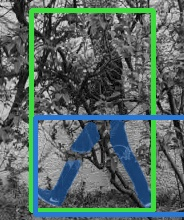
\includegraphics[height=8cm]{plots/nfo/bench_track.jpg} &
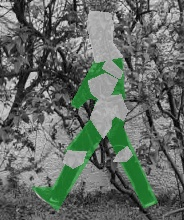
\includegraphics[height=8cm]{plots/nfo/bench_pixels.jpg} &
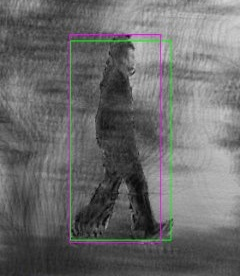
\includegraphics[height=8cm]{plots/nfo/bench_recog.jpg} \\[1mm]
\parbox[t]{6.9cm}{\centering\textbf{Tracking}\\\fontsize{19}{23}\selectfont success AUC, P@20 (LaSOT\,[7]): box
of the mask (blue) vs hand-drawn box (green)} &
\parbox[t]{6.9cm}{\centering\textbf{Segmentation}\\\fontsize{19}{23}\selectfont J (IoU), precision, recall vs
human labels} &
\parbox[t]{6.9cm}{\centering\textbf{Recognition}\\\fontsize{19}{23}\selectfont YOLO11\,[8] confidence, AP50 on a
masked integration}
\end{tabular}
\end{center}
\Unterschrift{Masked integration: 5 frames aligned by the motion of the hand-drawn boxes, averaged with the masks
as 0/1 weights. All design choices are made on scene 1; scenes 2--4 are only used for the final test.}

\Abschnitt{4\quad Contribution B: a method, Layer-SAM}

\textbf{Idea:} integrate evidence across \textbf{motion layers}\,[9]. Integrated with zero motion, frames give the
\textbf{empty scene}; aligned on the person's motion, the \textbf{integral image} (person sharp, foliage blurred).
Layer-SAM feeds both to SAM2.1 \emph{instead of} a memory.

\begin{center}
\resizebox{\linewidth}{!}{% Our architecture in the visual language of the SAM2 paper figure (plots/nfo/model_diagram.png):
% green = image encoder, orange = mask decoder, lavender = prompt encoder, pink = memory (not used).
% Blue outline = trained by us. Natural width ≈ 20 cm; the poster scales it to the column width.
\providecommand{\ArchSub}{\fontsize{14}{16}\selectfont}
% trained (flame) / frozen (snowflake) markers, drawn so they work with pdfLaTeX and XeTeX alike
\newsavebox{\FireBox}\newsavebox{\IceBox}
\sbox{\FireBox}{\tikz[baseline=-0.1em, x=0.9em, y=0.9em]{%
  \fill[orange!90!red] (0,-0.5) .. controls (-0.55,-0.25) and (-0.35,0.25) .. (0,0.75)
                       .. controls (0.35,0.25) and (0.55,-0.25) .. (0,-0.5);
  \fill[yellow!85!orange] (0,-0.45) .. controls (-0.25,-0.25) and (-0.15,0.05) .. (0,0.25)
                          .. controls (0.15,0.05) and (0.25,-0.25) .. (0,-0.45);}}
\sbox{\IceBox}{\tikz[baseline=-0.1em, x=0.9em, y=0.9em, line width=0.12em, cyan!60!blue, line cap=round]{%
  \foreach \a in {0,60,120} {\draw (\a:-0.55) -- (\a:0.55);
    \draw (\a:0.32) -- ++(\a+35:0.18); \draw (\a:0.32) -- ++(\a-35:0.18);
    \draw (\a:-0.32) -- ++(\a+215:0.18); \draw (\a:-0.32) -- ++(\a+145:0.18);}}}
\providecommand{\Fire}{\usebox{\FireBox}}\providecommand{\Ice}{\usebox{\IceBox}}
\definecolor{SamEnc}{HTML}{D4F5C4}\definecolor{SamEncD}{HTML}{8FCF79}
\definecolor{SamDec}{HTML}{FDE6C8}\definecolor{SamDecD}{HTML}{E9B676}
\definecolor{SamPrm}{HTML}{DEDDFB}\definecolor{SamPrmD}{HTML}{9E9BE6}
\definecolor{SamMem}{HTML}{F9DDF0}\definecolor{SamMemD}{HTML}{E7A9D3}
\begin{tikzpicture}[x=1cm, y=1cm, font=\fontsize{19}{22}\selectfont,
    lab/.style={align=center, font=\fontsize{17}{20}\selectfont},
    small/.style={align=center, font=\fontsize{14}{16}\selectfont, text=black!70},
    blk/.style={rounded corners=7pt, line width=1.4pt, align=center, minimum height=1.9cm},
    ours/.style={blk, draw=ColOurs, fill=ColOurs!14, line width=2.6pt},
    stride/.style={draw=ColOurs, fill=white, rounded corners=4pt, line width=1.2pt, minimum width=2.3cm,
                   minimum height=1.1cm, font=\fontsize{15}{17}\selectfont},
    arr/.style={-{Latex[length=4mm, width=3mm]}, line width=1.8pt, draw=black!80},
    thin/.style={-{Latex[length=3mm, width=2.4mm]}, line width=1.2pt, draw=ColOurs},
    feat/.style={draw=SamEncD, fill=SamEnc!70, line width=1.1pt, minimum width=1.3cm, minimum height=1.3cm}]

  % inputs
  \node[inner sep=0pt] (X) at (-6, 0) {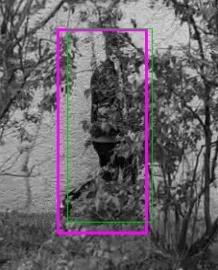
\includegraphics[height=4.2cm]{plots/nfo/inputs_0.jpg}};
  \node[inner sep=0pt] (C) at ( 0, 0) {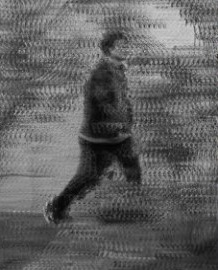
\includegraphics[height=4.2cm]{plots/nfo/inputs_2.jpg}};
  \node[inner sep=0pt] (B) at ( 6, 0) {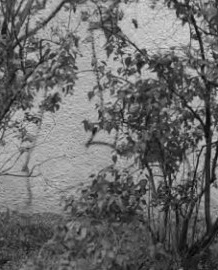
\includegraphics[height=4.2cm]{plots/nfo/inputs_1.jpg}};
  \node[lab, above=1mm of X] {\textbf{frame} $t$\\[-1mm]{\ArchSub with tracker box}};
  \node[lab, above=1mm of C] {\textbf{integral image}\\[-1mm]{\ArchSub 6 past frames, aligned}};
  \node[lab, above=1mm of B] {\textbf{empty scene}\\[-1mm]{\ArchSub encoded once per scene}};

  % shared image encoder (trapezoid, as in SAM2)
  \node[trapezium, trapezium angle=78, shape border rotate=180, draw=SamEncD, fill=SamEnc, line width=1.4pt,
        minimum width=18.5cm, minimum height=2cm, align=center] (enc) at (0, -3.9)
        {\Ice\ \textbf{image encoder}\\[-1mm]{\ArchSub same weights for all three}};
  \foreach \n/\x in {X/-6, C/0, B/6} \draw[arr] (\n.south) -- (\x, -2.9);

  % feature maps (strides 16 / 8 / 4)
  \foreach \n/\x/\t in {fx/-6/t, fc/0/I, fb/6/E} {
    \node[feat] at (\x+0.25, -6.5+0.25) {};
    \node[feat] (\n) at (\x, -6.5) {$F_{\t}$};
    \draw[arr] (\x, -4.9) -- (\n.north);
  }
  \node[small, anchor=west] at (7.0, -7.45) {strides\\16, 8, 4};

  % adapter: takes only the three feature maps; per stride, coarse to fine
  \node[ours, minimum width=15cm, minimum height=3.6cm] (ad) at (1, -9.9) {};
  \node[anchor=north west, align=left] at ([xshift=3mm, yshift=-2mm]ad.north west)
        {\Fire\ \textbf{adapter}\ \ {\ArchSub 0.7\,M parameters}};
  \node[stride] (s16) at (-3.2, -10.6) {stride 16};
  \node[stride] (s8)  at ( 0.9, -10.6) {stride 8};
  \node[stride] (s4)  at ( 5.0, -10.6) {stride 4};
  \draw[thin] (s16) -- (s8); \draw[thin] (s8) -- (s4);
  \foreach \n in {fx, fc, fb} \draw[arr] (\n.south) -- (\n.south |- ad.north);

  % corrections added to the frame features at each stride
  \node[circle, draw=black!80, line width=1.8pt, minimum size=1cm, inner sep=0pt,
        font=\fontsize{28}{28}\selectfont\bfseries] (plus) at (-9.6, -9.9) {$+$};
  \draw[arr] (fx.west) -| (plus.north);
  \draw[arr] (ad.west) -- node[above, small] {corrections} (plus.east);

  % decoder + prompt encoder
  \node[blk, draw=SamDecD, fill=SamDec, minimum width=7.2cm] (dec) at (-4.6, -13.6)
        {\Ice\ \textbf{mask decoder}};
  \node[blk, draw=SamPrmD, fill=SamPrm, minimum width=6.4cm] (pe) at (5, -13.6)
        {\Ice\ \textbf{prompt encoder}};
  \draw[arr] (plus.south) |- (dec.west);
  \draw[arr] (pe.west) -- (dec.east);
  \draw[arr, dashed] (pe.north |- ad.south) -- node[right, small] {point\\[-1mm]correction} (pe.north);

  % tracker: where to look
  \node[blk, draw=ColOurs, fill=white, line width=1.4pt, minimum width=6.4cm] (trk) at (5, -16.5)
        {\textbf{tracker}\\[-1mm]{\ArchSub motion + box: where to look}};
  \draw[arr] (trk.north) -- (pe.south);
  % tracker input: change of the frame features against the empty scene
  \draw[-{Latex[length=3mm, width=2.4mm]}, line width=1.2pt, draw=black!60] (fb.east) -- (9.2, -6.5) -- (9.2, -15.9)
        node[pos=0.5, rotate=-90, anchor=south, inner sep=1.5pt, small] {change of $F_t$ vs $F_E$} -- ([yshift=6mm]trk.east);
  % the tracker's motion builds the integral image
  \draw[arr, draw=ColOurs, dashed] (trk.east) -- ++(1.6, 0) |- ([yshift=3.4cm]C.north) node[pos=0.75, above, small, text=ColOurs]
        {motion: aligns the past frames} -- ([yshift=1.75cm]C.north);
  % legend
  \node[anchor=south west, align=left, font=\fontsize{16}{19}\selectfont] at (-11.6, -21.4)
        {\Fire\ trained (ours)\\ \Ice\ frozen SAM2.1};

  % output
  \node[inner sep=0pt] (M) at (-4.6, -18.1) {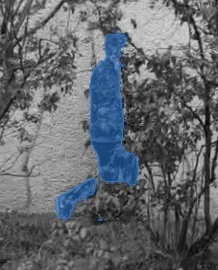
\includegraphics[height=4.2cm]{plots/nfo/inputs_6.jpg}};
  \draw[arr] (dec.south) -- (M.north);
  \node[lab, left=2mm of M] {\textbf{mask}};

  % memory path of SAM2: not used
  \node[blk, draw=SamMemD, fill=SamMem!50, dashed, minimum width=6.4cm, text=black!55] (mem) at (5, -19.4)
        {memory of past masks\\[-1mm]{\ArchSub not used}};
  \draw[arr, draw=black!35, dashed] (M.east |- mem.west) -- node[text=ColSamurai, font=\fontsize{30}{30}\selectfont\bfseries]
        {$\times$} (mem.west);
\end{tikzpicture}
}
\end{center}

With a static camera the empty scene is encoded once per scene: two encoder passes per frame, 61 vs 53\,ms for
SAM2.1 with memory.

% REVIEW: what is the deeper idea behind the training? (asymmetric penalty + ambiguity band; not scene geometry)
% REVIEW: is choosing a recall-leaning loss circular w.r.t. the downstream metrics? (it was selected on scene-1
%         hand labels, not on tracking/recognition; is there a better first-principles reason for extent over caution?)
\Abschnitt{5\quad Training: extent over caution}

A missed fragment is evidence lost for good (smaller box, weaker integration); a foliage pixel at the person's edge
costs little. So the loss is asymmetric.

\Bild{plots/nfo/synth_row.jpg}
\Unterschrift{Synthetic clips with exact visible masks (GPJATK people, procedural foliage, CanaTree100\,[10]):
frame, person, visible target, loss weights.}

\textbf{Loss:} focal\,[11] + \textbf{Focal Tversky}\,[12] (from medical segmentation of small structures): misses
weigh more than false alarms. No loss in the ambiguous band next to visible fragments (yellow). Chosen on
scene-1 hand labels (IoU), not on the downstream metrics.

%======================================================================= column 3: results
\columnbreak
\Abschnitt{6\quad Results on NFO-VOS}

\begin{center}
\setlength{\tabcolsep}{3.6pt}\fontsize{20}{25}\selectfont
\begin{tabular}{@{}l cc ccc ccc@{}}
 & \multicolumn{2}{c}{\textbf{tracking}} & \multicolumn{3}{c}{\textbf{segmentation}} & \multicolumn{3}{c}{\textbf{recognition}} \\
 & AUC & P@20 & J & P & R & conf & IoU & AP50 \\\hline
SAM2.1 & .571 & .682 & .733 & \textbf{.89} & .80 & .666 & .692 & .869 \\
SAMURAI & .579 & .691 & .730 & .88 & .81 & .663 & .696 & .863 \\
SAM2.1 + tracker$^*$ & .661 & .766 & .745 & .82 & \textbf{.88} & .636 & .691 & .861 \\
SAM2.1, no memory$^*$ & .628 & .727 & .685 & .80 & .83 & .596 & .645 & .814 \\
\textbf{ours, no memory} & \textbf{.678} & \textbf{.773} & \textbf{.756} & .86 & .85 & \textbf{.667} & \textbf{.705} & \textbf{.878}
\end{tabular}
\end{center}
\Unterschrift{32 walks, 4 scenes (scenes 2--4 alone: same conclusions); J/P/R on the hand-labelled frames; ours:
mean of 3 seeds. Recognition IoU: top YOLO detection vs hand-drawn box.\\
$^*$prompted in every frame by our tracker; ``no memory'': SAM2.1's image model.}

\Merke{No memory, yet above every memory variant on tracking, segmentation and recognition. Better memory
management (SAMURAI) adds little here.}

\Unter{Masks: SAM2.1 vs ours}
\Bild{plots/nfo/qual.png}
\Unterschrift{Two frames of one walk in scene 4. \emph{right}: precision; \emph{finds}: recall.}

\Unter{Does the segmentation degrade over time?}
\Bild{plots/nfo/masksize.png}
\Unterschrift{Mask area / box area, relative to frame 6 (median, 95\,\% CI). Prompted only at the start, memory masks
shrink (0.76$\times$ ours after frame 30); with tracker prompts they keep their size, as ours do.}

\Unter{Ablation}
\Bild{plots/nfo/ablation.png}
\Unterschrift{From SAM2.1 to ours, one change per row; lines: 95\,\% CI, dots: 3 seeds. Without the integral image, the
adapter gets the empty scene in its place.}

\Unter{Recognition vs.\ frames integrated}
\Bild{plots/nfo/recogN.png}
\Unterschrift{YOLO11 AP50, N masked frames integrated: on par up to N\,=\,7 (N\,=\,5 in the table), ahead beyond; $^*$as in the table.}

\end{multicols*}


\clearpage

\end{document} % !!! NICHT ENTFERNEN !!!
